
\section{Introduction}

In the previous Chapters I studied the effect that adding positive feedback loops to the genetic toggle switch has on the robustness of the system. I found that adding two positive feedback loops to the simple toggle switch can increase its parametric robustness. The next step in this analysis would be to test these predictions experimentally. Therefore, in this Chapter I provide the experimental design for the construction of the genetic toggle switch with single and double positive autoregulation. The newly constructed switches could then be compared to the simple ~\textcite{Litcofsky:2012gr} toggle switch experimentally. Their robustness could be tested by varying the experimental conditions, like temperature and pH, and measuring the response of the switch.

Structurally, this Chapter is organised as follows: First I provide an overview of the cloning plan, by listing the relevant BioBrick parts used and their interactions. Then I outline the experimental design for producing these switches.


\section{Cloning overview}

The~\textcite{Litcofsky:2012gr} toggle switch plasmid, pKDL071, used in Chapter (XXX) is modified to construct three new switches. Two switches will have single positive autoregulation, one on each gene, and one switch will have positive autoregulation on both genes. An overview of the cloning stages to be carried out is shown in Figure~\ref{fig:plan}. The three stages required for the cloning plan to be completed are outlined in the sections below. 

\begin{figure*}[t]
	\begin{center}
		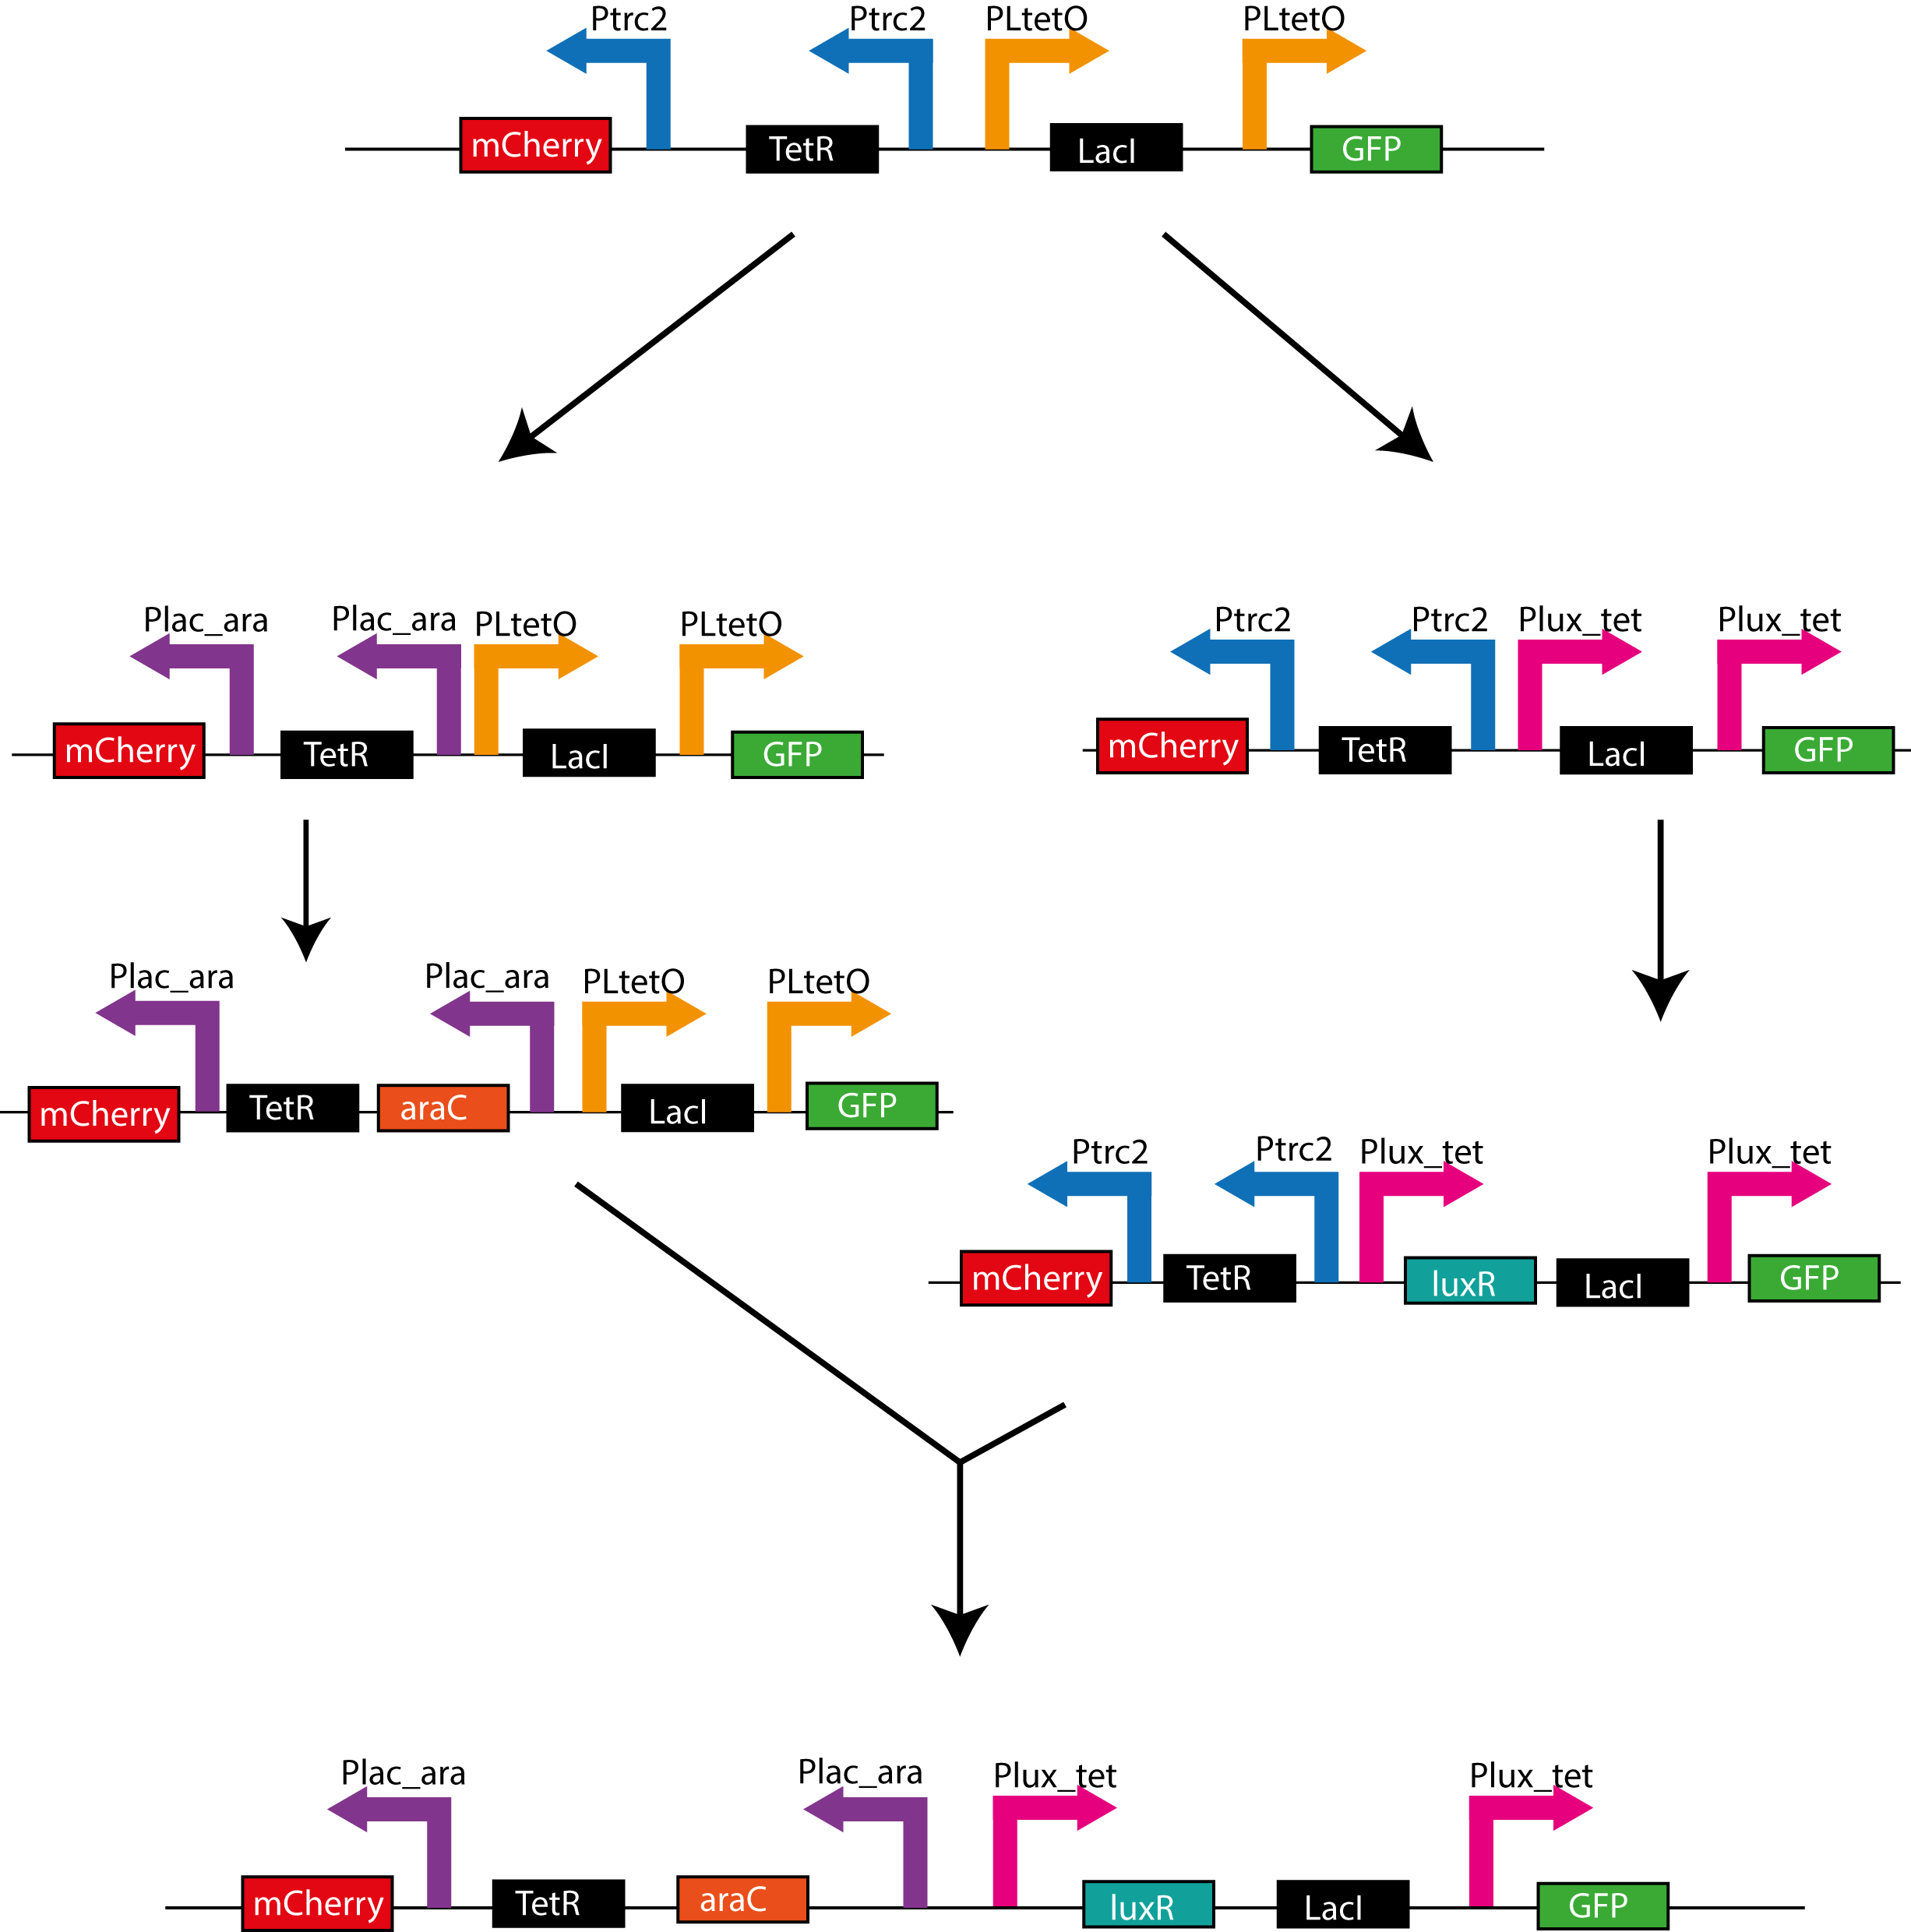
\includegraphics[scale=0.7]{../../chapters/chapterDesignSwitches/images/switches_cloning_big.png}
		\caption[LoF caption]{\label{fig:plan}: An overview of the cloning plan to produce three new switches, two with single positive autoregulation and one with double positive autoregulation.}
	\end{center}
\end{figure*}
\clearpage

\subsection{Resulting switches}
The three switches shown in Figure~\ref{fig:finalpl} will be constructed through this cloning process. The first switch, on plasmid pKDL071-plac/ara-araC is a toggle switch with positive autoregulation on the TetR/mCherry side of the switch. The second plasmid, pKDL071-pLuxTet-luxR consists of a toggle switch with positive autoregulation on the LacI/GFP side of the switch. Finally, the switch with positive autoregulation on both sides of the switch is on the pKLD0713a plasmid. The plasmid maps and a schematic of their components' interactions are shown in Figure~\ref{fig:finalpl}. 

\begin{figure*}[htbp]
	\begin{center}
		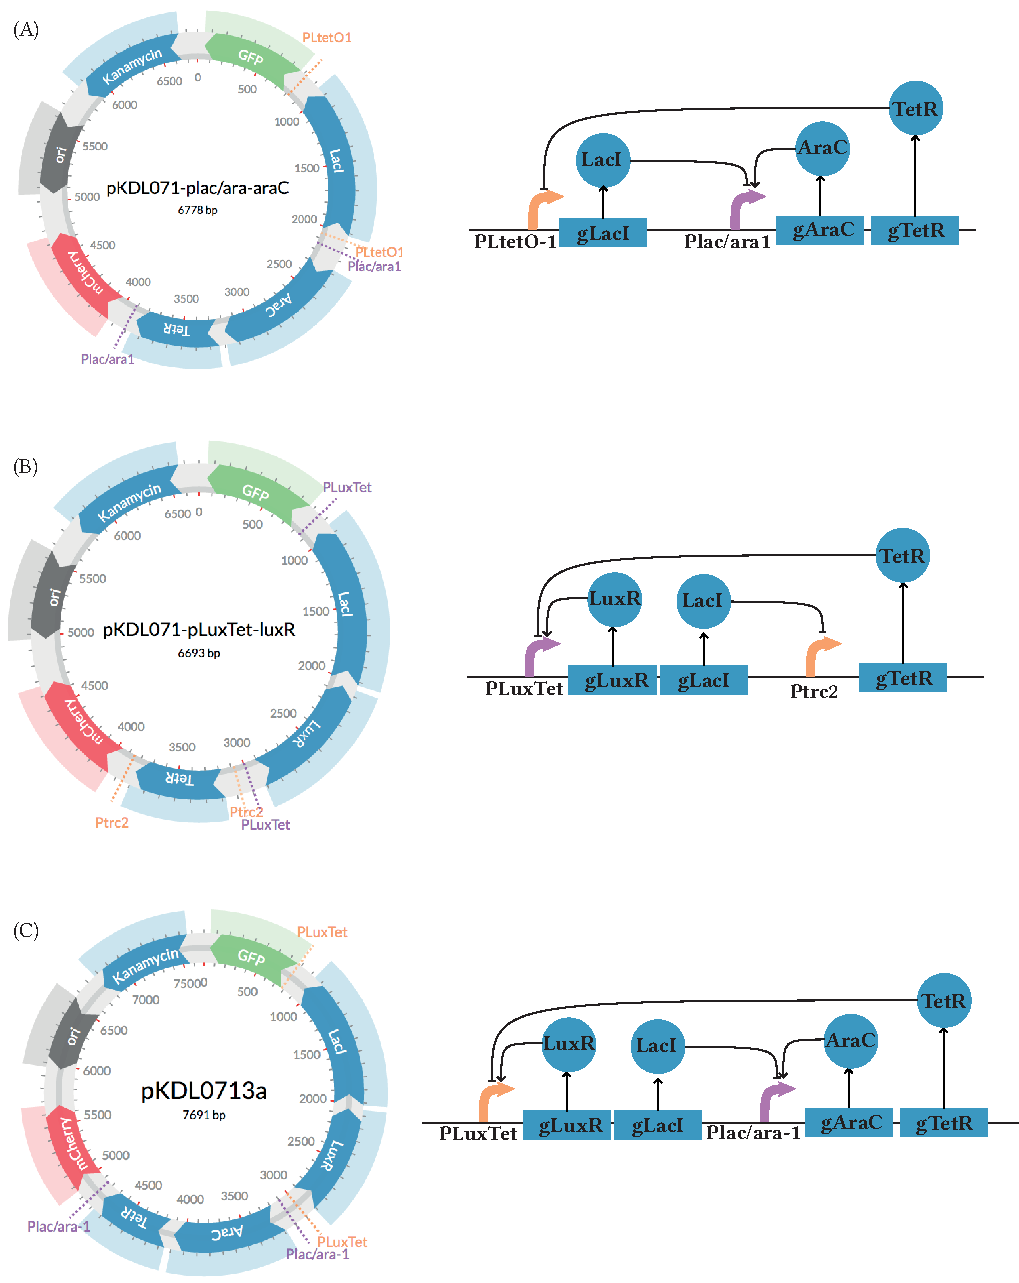
\includegraphics[scale=0.7]{../../chapters/chapterDesignSwitches/images/final-plasmids.pdf}
		\caption[LoF caption]{\label{fig:finalpl}: The plasmid maps of three new switches to be constructed. The first two switches have a single positive autoregulation on each side of the switch respectively. The switch on the far right has positive autoregulation on both genes. }
	\end{center}
\end{figure*}

\section{Experimental design}

The construction of the three switches shown in Figure~\ref{fig:finalpl} is broken down in three stages, one for the construction of each switch. In this section I will outline the necessary cloning steps that need to be carried out in order to construct each switch. The detailed methods that will have to be used for each cloning step are described in Section (XXX). All primer sequences have been designed and are given in Appendix (XXX). Following the construction of each plasmid outlined below, competent \textit{E.coli} cells will be transformed following the method outlined in Section (XXX).

\subsection{Stage 1 - Construction of pKDL071-plac/ara-araC}

In order to construct plasmid pKDL071-plac/ara-araC with single positive autoregulation on the mCherry/TetR side, the P\textsubscript{trc2} promoter will be swapped for the P\textsubscript{lac\_ara-1} and AraC added upstream of TetR. P\textsubscript{lac\_ara-1} is activated by arabinose (AraC) and repressed by LacI~\autocite{Lutz:1997ti}, and is thus ideal. The P\textsubscript{lac\_ara-1} promoter is present in the pJS167 plasmid, which is provided by Jeff Hasty (Addgene plasmid \# 48881)~\autocite{Stricker:2008jqa}. This promoter is also present in the BioBrick registry of standard biological parts as BBa\_K1713000. 



\begin{figure*}[t]
	\begin{center}
		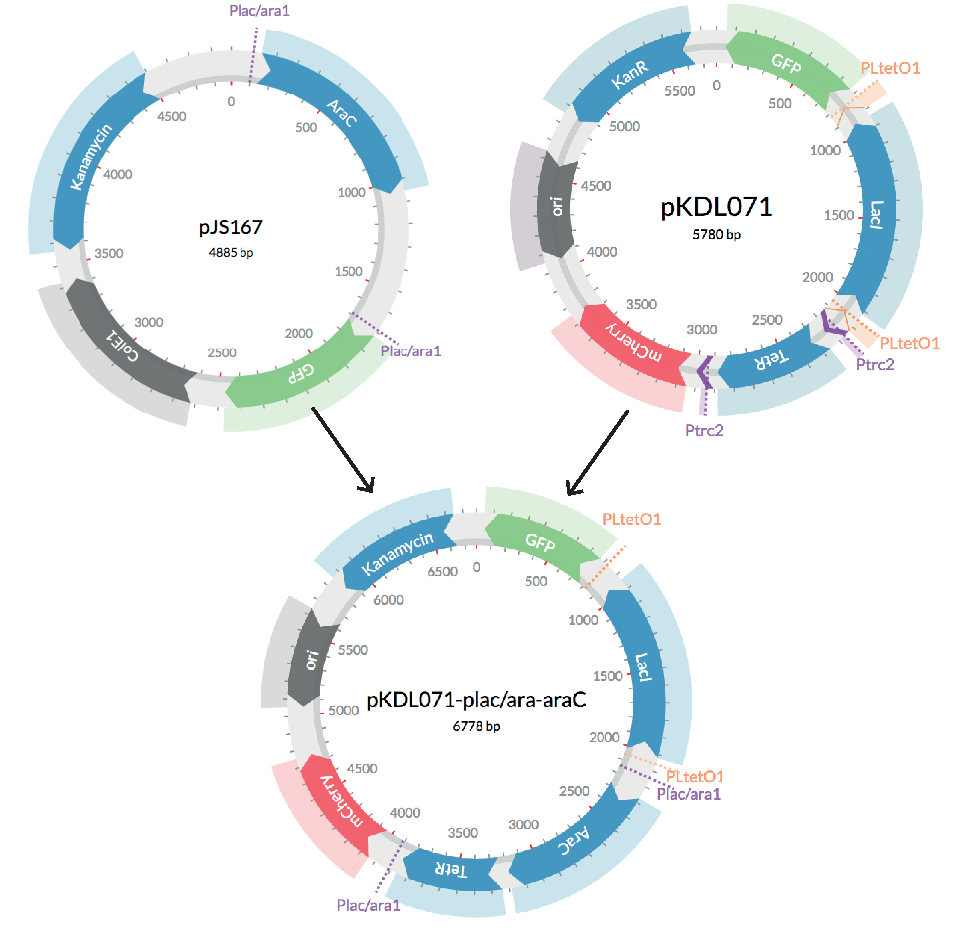
\includegraphics[scale=0.7]{../../chapters/chapterDesignSwitches/images/stage1_cloning.pdf}
		\caption[LoF caption]{\label{fig:stage1}: Stage 1 cloning procedure. The pKDL071-plac/ara-araC plasmid is constructed via PCR cloning from the pJS167 and pKDL071 plasmids.}
	\end{center}
\end{figure*}
\clearpage

Using \acrshort{pcr} cloning, the P\textsubscript{lac\_ara-1} promoter will be cloned from pJS167, with added XmaI and KasI  restriction enzyme sequences on each end. Both pKDL071 and the \acrshort{pcr} product will be digested with XmaI and KasI restriction enzymes. After gel electrophoresis and gel extraction, the two will be subsequently ligated. The resulting plasmid should have the P\textsubscript{lac\_ara-1} promoter instead of the P\textsubscript{trc2} promoter upstream of mCherry.


Following that, PCR cloning will be used to clone  P\textsubscript{lac\_ara-1} and AraC from the pJS167 plasmid. EagI and SalI flanking sequences will be added via PCR on the 5' and 3' ends. Plasmid pKDL071 and the PCR product will be digested using EagI and SalI. Following gel electrophoresis and gel extraction, the two products will be ligated in order to complete the pKDL071-plac/ara-araC plasmid. The detailed methods for each cloning technique mentioned here can be found in Section (XXX).


\subsection{Stage 2 - Construction of pKDL071-pluxtet-luxR}
\label{sec:stage2}


In order to construct the plasmid pKDL071-pluxtet-luxR, the P\textsubscript{Lux/tet} promoter is necessary. The P\textsubscript{Lux/tet} promoter is present in the BioBrick registry of standard biological parts as BBa\_K934024. P\textsubscript{Lux/tet} is a hybrid promoter activated by LuxR and repressed by TetR. This promoter will be added in exchange of P\textsubscript{LtetO-1} to the pKDL071 plasmid. The LuxR gene will also added upstream of LacI, in order to construct a switch with positive autoregulation on the LacI/GFP side. 

%\subsubsection{pLux/tet synthesis}
First, the P\textsubscript{Lux/tet} promoter is synthesised. The reverse complement of BBa\_K934024 with added flanking sequences of EcoO1091 and SphI on the 5' side and AclI and Eag1 at the 3' side. These are added to aid with further cloning steps. The sequence synthesised is given below:

\vspace{3 mm}
\noindent 5'- TTGGGACCTGCATGCTAATCTCTATCACTGATAGGGATAATACGAGTATCTC\\TATCACTGATAGGGAGTAAACCTGTACGATCCTACAGGTAACGTTCGGCCG -3'
\vspace{3 mm}

The pLux/tet and pKDL071 plasmids will subsequently be digested with SphI and AclI. Following gel extraction and ligation, the P\textsubscript{Lux/tet} promoter will be added upstream of GFP, replacing the P\textsubscript{LtetO-1} promoter. Then, the plux/tet and pKDL071 plasmids will be digested with EcoO109I and EagI restriction enzymes. Following gel extraction and digestion, the P\textsubscript{Lux/tet} promoter will be added upstream to LacI, replacing the P\textsubscript{LtetO-1} promoter. 


The final stage of constructing the pKDL071-pluxtet-luxR plasmid consists of PCR cloning of the pTD103aiiA(Cm) plasmid with added BsGI flanking sequences at both ends. The pTD103aiiA(Cm) is provided by Jeff Hasty (Addgene plasmid \# 48886)~\autocite{Prindle:2012cj}. The plasmid constructed in the previous step and the PCR product will be digested with BsGI restriction enzyme. Following gel extraction and ligation, the pKDL071-pluxtet-luxR should be complete. The ligated products will be transformed into thermocompetent \textit{E.coli}.


\begin{figure*}[htbp]
	\begin{center}
		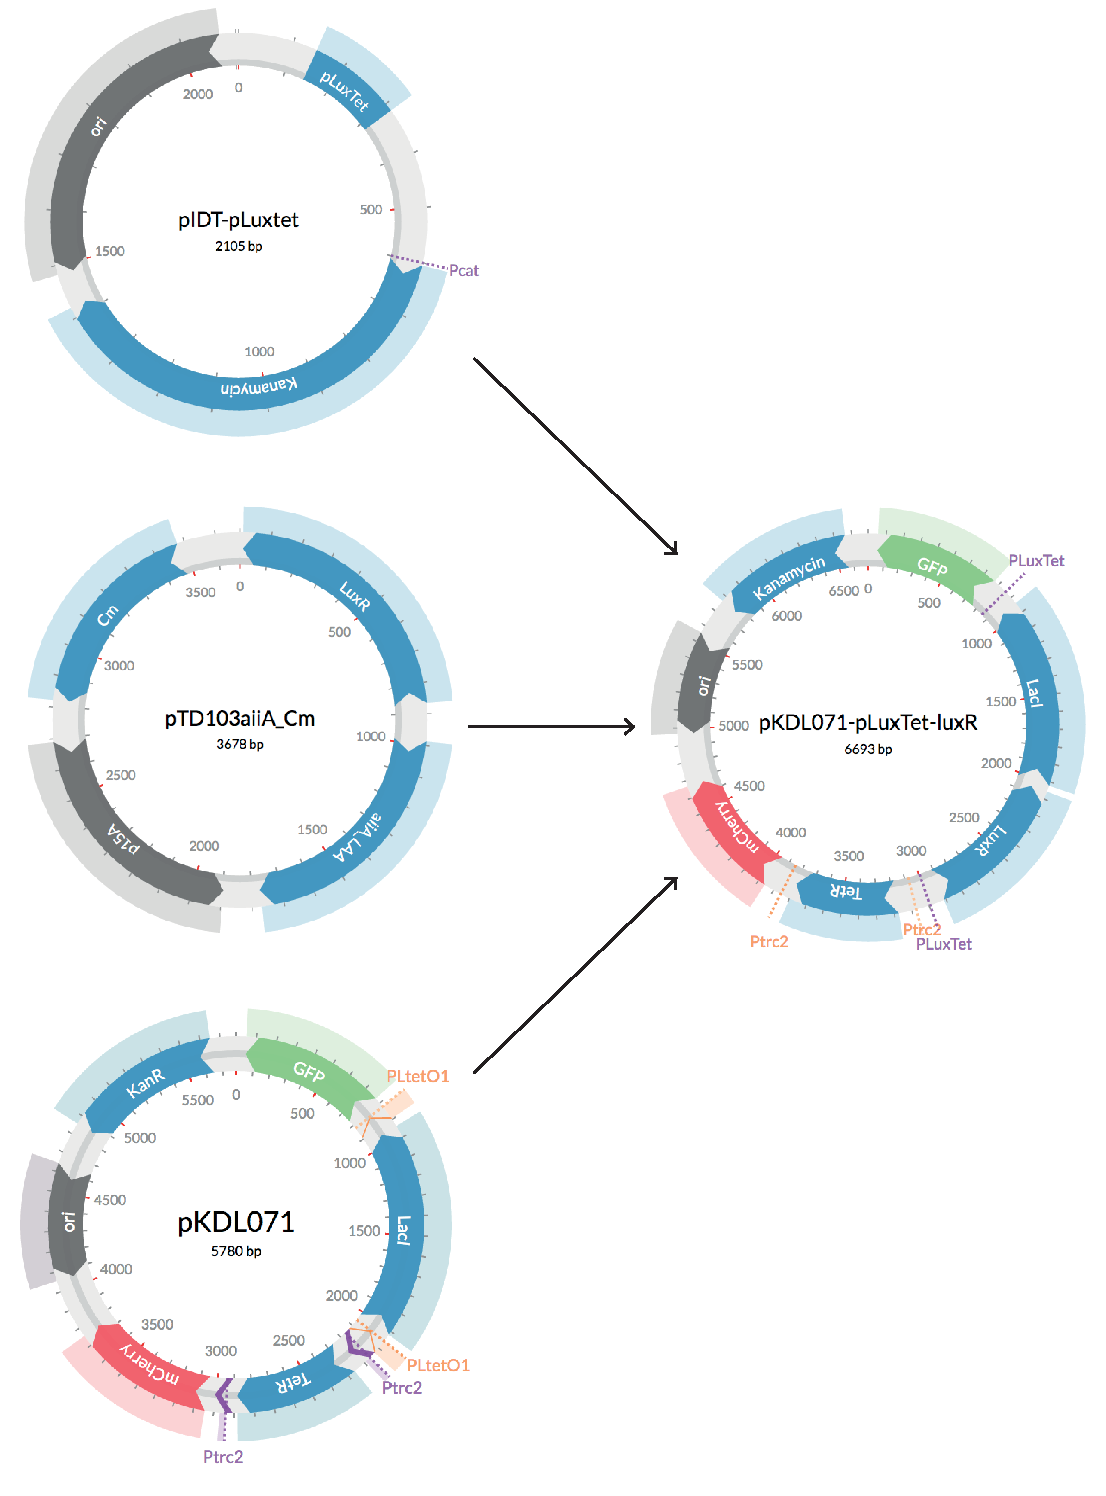
\includegraphics[scale=0.6]{../../chapters/chapterDesignSwitches/images/stage2_cloning.pdf}
		\caption[LoF caption]{\label{fig:stage2}: Stage 2 cloning procedure. The pKDL071-pluxtet-luxR  plasmid is constructed via PCR cloning from the synthesised P\textsubscript{Lux/tet} promoter, pKDL071 and pTD103aiiA(Cm) plasmids.}
	\end{center}
\end{figure*}

\subsection{Stage 3 - Construction of pKDL0713a}

The final construction stage requires the complete pKDL071-plac/ara-araC plasmid, as well as the synthesised P\textsubscript{Lux/tet} promoter and pTD103aiiA(Cm) plasmid used in Stage 2. 

 The plux/tet plasmid and pKDL071-plac/ara-araC will be digested with SphI and AclI restriction enzymes. This will be followed by gel extraction to isolate the fragments of interest. These will then be ligated to result in the modified pKDL071-plac/ara-araC plasmid, (pKDL071-plac/ara-araC-pluxtetA) with P\textsubscript{Lux/tet}upstream of GFP instead of P\textsubscript{LtetO-1}.
 
Then, the plux/tet plasmid and the plasmid created above (pKDL071-plac/ara-araC-pluxtetA) will be digested with EcoO109I and EagI. Following gel extraction and ligation, the P\textsubscript{Lux/tet} promoter will be added upstream of LacI instead of P\textsubscript{LtetO-1} to make a new plasmid, pKDL071-plac/ara-araC-pluxtet. Subsequently, the PCR product produced above of pTD103aiiA\_Cm with BsGI flanking sequences and pKDL071-plac/ara-araC-pluxtet will be digested using BsGI. The fragments of interest will then be extracted following gel electrophoresis of the digested products and ligated. The ligates should be screened for the correct orientation of the insert. 


\begin{figure*}[htbp]
	\begin{center}
		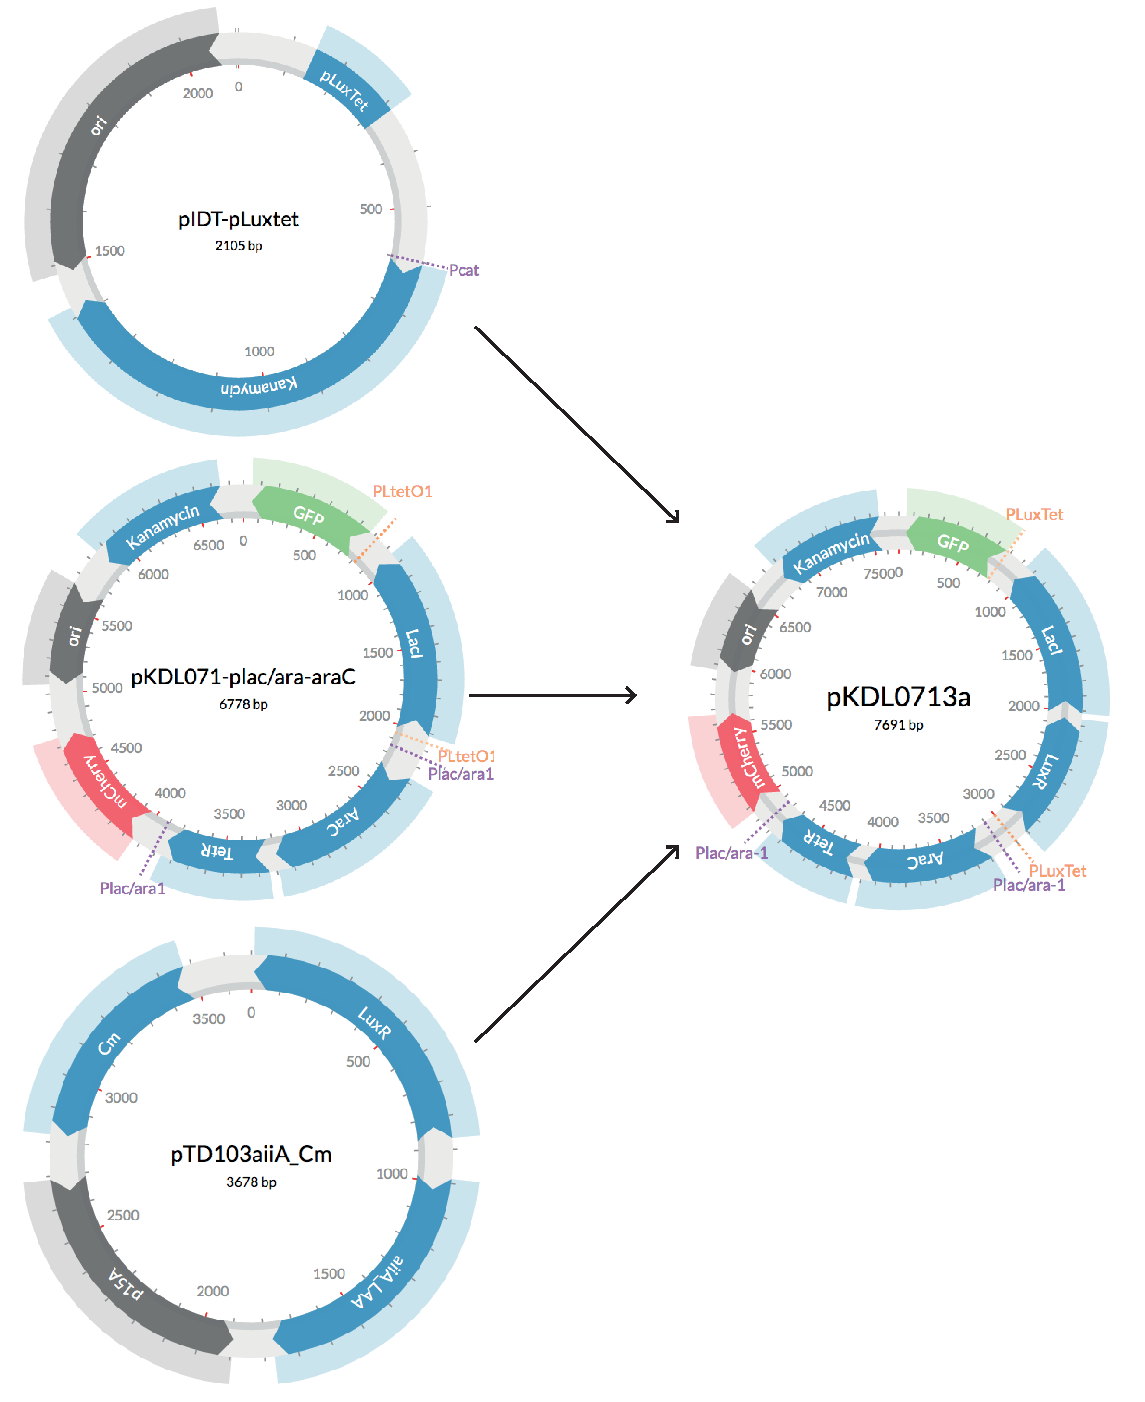
\includegraphics[scale=0.7]{../../chapters/chapterDesignSwitches/images/stage3_cloning.pdf}
		\caption[LoF caption]{\label{fig:stage3}: Stage 3 cloning procedure. The pKDL0713a plasmid is constructed via PCR cloning from the synthesised P\textsubscript{Lux/tet} promoter, pKDL071-plac/ara-araC and pTD103aiiA(Cm) plasmids.}
	\end{center}
\end{figure*}
\clearpage

%\begin{figure*}[t]
%	\begin{center}
%		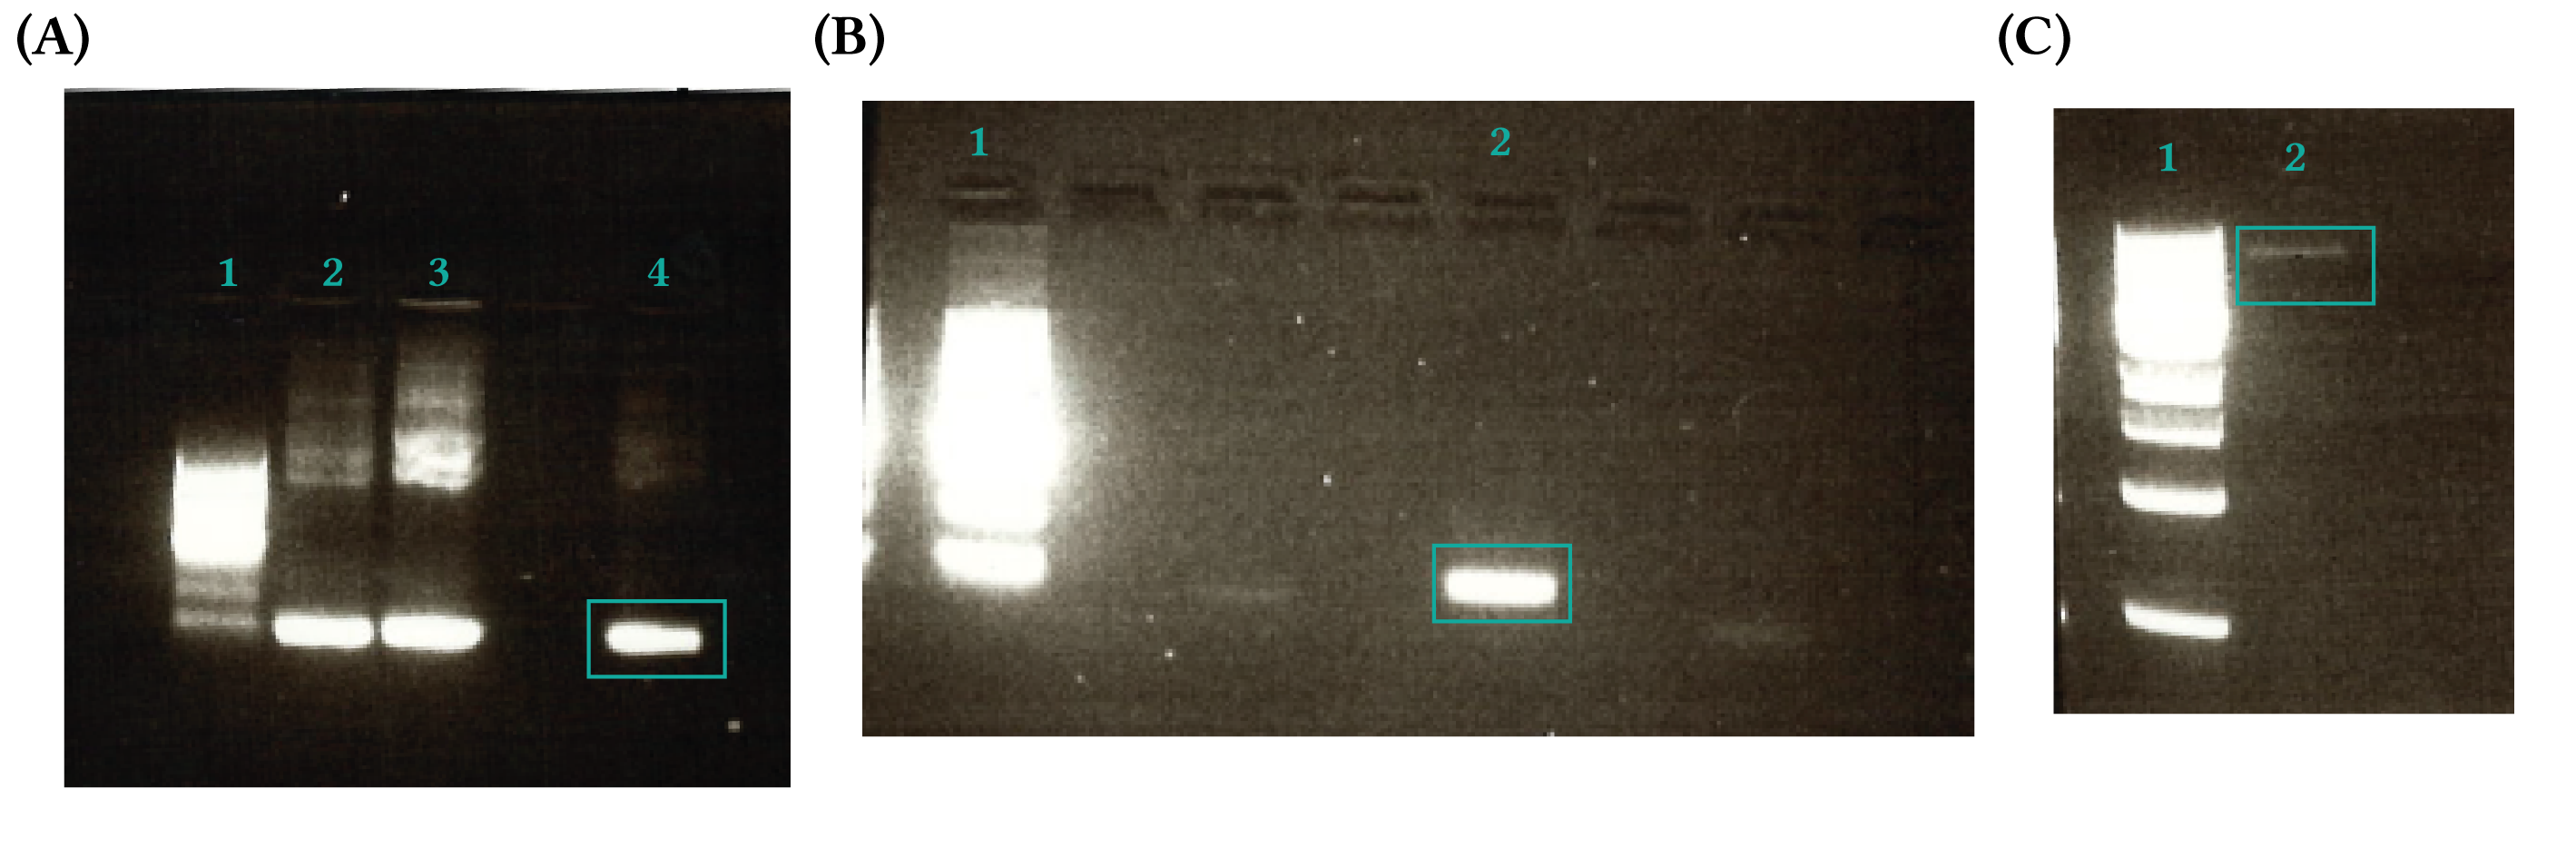
\includegraphics[scale=0.6]{../../chapters/chapterDesignSwitches/images/illustrator/gels/plac_ara_tetR.png}
%		\caption[LoF caption]{\label{fig:plac_ara_tetr_gels}:(A) \acrshort{pcr} result of plasmid pJS167, to clone the P\textsubscript{lac\_ara-1} promoter. (A.1) The 100bp DNA ladder, (A.2-A.4) three repeats of the \acrshort{pcr}. (B) \acrshort{pcr} product digestion with NcoI and SalI. (B.1) The 100bp DNA ladder. (B.2) Digested PCR product. (C) pKDL071 digestion with NcoI and SalI. (C.1) The 1KB DNA ladder. (C.2) The digested plasmid.}
%	\end{center} 
%\end{figure*}


%\begin{figure*}[t]
%	\begin{center}
%		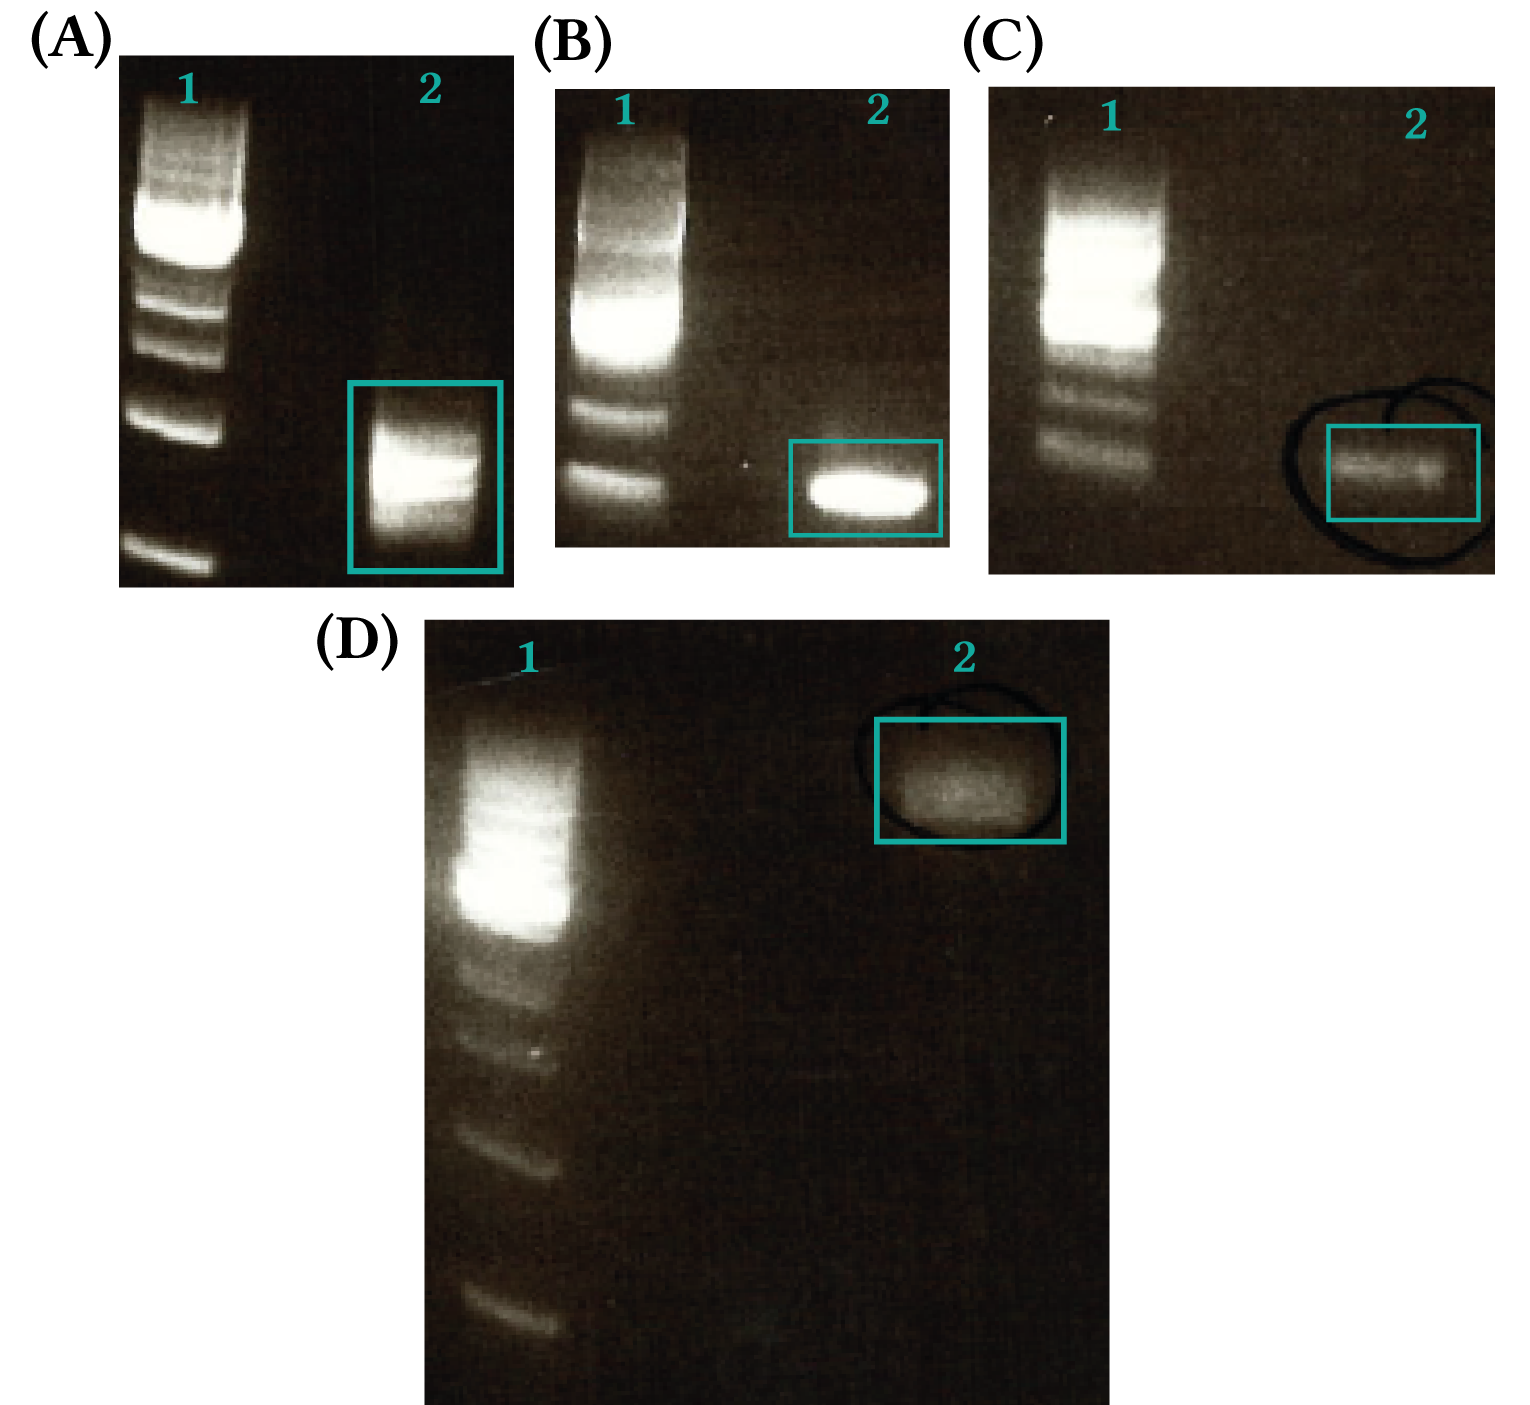
\includegraphics[scale=0.6]{../../chapters/chapterDesignSwitches/images/illustrator/gels/plac_ara_both-01.png}
%		\caption[LoF caption]{\label{fig:plac_ara_both_gels}:A) \acrshort{pcr} result of plasmid pJS167, to clone the P\textsubscript{lac\_ara-1} promoter with the AraC gene. (A.1) The 1KB DNA ladder, (A.2) the \acrshort{pcr} product. (B) \acrshort{pcr} result of plasmid pJS167, to clone the P\textsubscript{lac\_ara-1} promoter to be placed upstream of mCherry. (B.1) The 100bp DNA ladder. (C.1) The 100bp DNA ladder. (C.2) \acrshort{pcr} product digestion with XmaI and KasI. (C.3) pLuxTet digestion with SphI and AclI. (D.1) The 1KB DNA ladder. (D.2) pKDL071 digestion product with XmaI and KasI. (D.3) pKDL071 digestion product with SphI and AclI. }
%	\end{center}
%\end{figure*}

\clearpage
\section{Discussion}

I started implementing the experimental plan outlined above. In Stage 1 all the \acrshort{pcr}s and digestions described were completed successfully (data not shown). Transformation of the ligated products into thermocompetent \textit{E.coli} was carried out, but the transformation was not successful. In Stage 2 the P\textsubscript{Lux/tet} promoter was synthesised. Synthesis was carried out by Integrated DNA Technologies, Inc. (Leuven, Belgium, \url{http://eu.idtdna.com/CodonOpt}). \textit{E.coli} Dh5α was transformed with the synthesised plasmid. The method is outlined in Section(XXX). All subsequent \acrshort{pcr}s and digestions described in Section~\ref{sec:stage2} were carried out successfully. Due to time constraints, the rest of the experimental plan was not carried out.

%Following ligation and transformation into thermocompetent \textit{E.coli} Dh5α, the resulting plasmid was sequenced, which proved the cloning to be unsuccessful. Due to 


\section{Summary}

In this Chapter I designed the experimental protocol to be followed in order to construct three novel switches. These switches can be used in the future in synthetic biology applications. The execution of the experimental protocol described has not been completed to date but constitutes the future directions of this project.

